

\documentclass{article}
\usepackage{anyfontsize}
\usepackage{graphicx}
\usepackage{hyperref}
\usepackage{parskip}
\usepackage{enumitem}
\usepackage{array}
\usepackage{tabularx}
\usepackage[section]{placeins}
\usepackage{float}% If comment this, figure moves to Page 2
\usepackage[dvipsnames]{xcolor}
\usepackage{listings}
\usepackage{alloy-style}

\fontsize{10pt}{12pt}\selectfont % Set the font size
\begin{document}

% FRONT PAGE
\begin{titlepage}
    \begin{center}
        
        Politecnico di Milano\\
      
        Computer Science and Engineering\\
        
        Software Engineering II\\

        \vfill
        
        {\Large \textbf{Design Document - CodeKataBlade}}\\
        
        \vfill

        José Alejandro Sarmiento

        \today

        v1.0
        
    \end{center}
\end{titlepage}
\newpage


% TABLE OF CONTENTS
\tableofcontents
\newpage

% 1. INTRODUCTION
\section{INTRODUCTION}
\subsection{Purpose}

The purpose of this document is to provide a detailed description of the architecture of the system to be, CodeKataBlade, and to show how the requirements presented in the RASD document are met by the architecture. The document also contains the implementation, integration and test plan for the system.

\subsection{Scope}

CodeKataBlade is a software system designed to facilitate and enhance the practice of code katas, which are small coding exercises aimed at improving programming skills. The system provides a platform where educators can create tournaments and battles, and students can register, form teams, and submit their solutions to coding problems.

CodeKataBlade allows educators to create tournaments, which serve as spaces for organizing multiple battles. Educators can invite other educators to participate in tournaments and perform manual evaluations on the submissions of battles they own. The system also provides a leaderboard that is updated in real-time, displaying the rankings of participants based on their performance in the battles.

Students can register to tournaments and battles, either individually or as part of a team. They can submit their solutions to coding problems within the specified deadlines. The system automatically evaluates the submissions using build automation scripts and provides feedback to the students. A set of test cases is used to assess the correctness and efficiency of the solutions.

CodeKataBlade integrates with GitHub, a popular code hosting platform, allowing students to fork repositories and work on their solutions using version control. GitHub Actions, a CI/CD tool, is utilized to automate the evaluation process and provide continuous integration and delivery capabilities.

\subsection{Definitions, Acronyms, Abbreviations}

\subsubsection{Definitions}
 
\begin{itemize}
    \item \textbf{Tournament:} A tournament is a space where educators can create battles and students can register to them. It has a registration deadline and a leaderboard that is updated every time a battle ends.
    \item \textbf{Battle:} A battle is a space where students can register to and submit their solutions to a problem. It has a registration deadline, a final submission deadline, a leaderboard that is updated every time a new evaluation is performed and a set of test cases that will be used to evaluate the submissions.
    \item \textbf{GitHub:} GitHub is a code hosting platform for version control and collaboration. It lets you and others work together on projects from anywhere.
    \item \textbf{GitHub Actions:} GitHub Actions is a CI/CD tool that allows you to automate your software development workflows in the same place you store code and collaborate on pull requests and issues.
    \item \textbf{Educator:} An educator, in the context of the system, is a user of the platform that can create tournaments and battles, invite other educators to tournaments, perform manual evaluations on the submissions of a battle they own and consolidate the results of a battle.
    \item \textbf{Student:} A student, in the context of the system, is a user of the platform that can register to tournaments and battles, create teams and submit their solutions to a battle.
    \item \textbf{Build Automation Scripts:} Build automation scripts are scripts that are run automatically by the system every time a commit is pushed to the main branch of the forked repository of a battle. They are used to evaluate the submissions of the students.
    \item \textbf{Test Case:} A test case is a set of conditions under which a tester will determine whether an application, software system or one of its features is working as it was originally established for it to do.
    \item \textbf{Timeliness:} Timeliness is the quality of doing something or producing something at the right time. In the context of the system, it refers to the time in which a student submits their solution to a battle with respect to the start of the battle and the final submission deadline.
\end{itemize}

\subsubsection{Acronyms}

\begin{itemize}
    \item \textbf{CKB:} CodeKataBattle
    \item \textbf{S2B:} System to Be
    \item \textbf{TDD:} Test-Driven Development
    \item \textbf{CI/CD:} Continuous Integration/Continuous Delivery
    \item \textbf{UI:} User Interface
    \item \textbf{API:} Application Programming Interface
    \item \textbf{UML:} Unified Modeling Language
\end{itemize}

\subsubsection{Abbreviations}

\begin{itemize}
    \item \textbf{Gn:} Goal number n
    \item \textbf{Wn:} World Phenomena number n
    \item \textbf{SPn:} Shared Phenomena number n
    \item \textbf{Dn:} Domain Assumption number n
    \item \textbf{Rn:} Requirement number 
    \item \textbf{UCn:} Use Case number n
\end{itemize}

\subsection{Revision history}
\subsection{Reference Documents}

The specification of the RASD and DD assignment of the Software
Engineering II course, held by professor Matteo Rossi, Elisabetta Di Nitto and
Matteo Camilli at the Politecnico di Milano, A.Y 2023/2024.

\subsection{Document Structure}

\begin{itemize}
    \item \textbf{1. Introduction:} This section provides an overview of the entire document. It describes the purpose and scope of the system, the definitions, acronyms and abbreviations used in the document, the revision history and the reference documents.
    \item \textbf{2. Architectural Design:} This section describes the architecture of the system. It provides an overview of the high-level components and their interaction, the component view, the deployment view, the runtime view, the component interfaces, the selected architectural styles and patterns and other design decisions.
    \item \textbf{3. User Interface Design:} This section provides a mockup of the user interface of the system.
    \item \textbf{4. Requirements Traceability:} This section describes how the requirements defined in the RASD map to the design elements defined in this document.
    \item \textbf{5. Implementation, Integration and Test Plan:} This section describes the order in which the components of the system will be implemented, integrated and tested.
    \item \textbf{6. Effort Spent:} This section describes the amount of time spent by each group member to redact this document.
    \item \textbf{7. References:} This section provides a list of the reference documents used to redact this document. 
\end{itemize}

% 2. ARCHITECTURAL DESIGN
\section{ARCHITECTURAL DESIGN}
\subsection{Overview: High-level components and their interaction}

\begin{figure}[H]
    \centering
    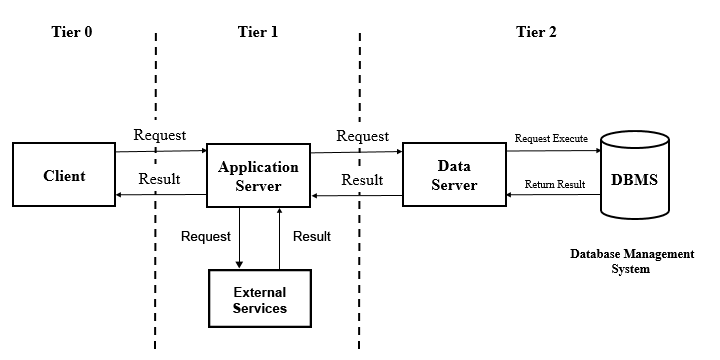
\includegraphics[width=1\textwidth]{images/3-tier-architecture.png}
    \caption{Three-tier Architecture}
    \label{fig:3-tier-architecture}
\end{figure}
The chosen architecture for the system is a three-tier architecture, a widely adopted
model for developing scalable and maintainable web applications. This architectural 
style divides the application into three interconnected layers: presentation, application, 
and data, with the addition of the external services like GitHub and email services.
The rationale behind selecting this architecture is to achieve separation of concerns, 
modularity, and scalability.

\subsubsection*{Presentation Layer}

The presentation layer constitutes the user interfaces for both students and educators, 
encompassing web or mobile interfaces. It is responsible for user interactions, 
displaying data, and triggering actions within the system.

\subsubsection*{Application Layer}

The application layer serves as the business logic layer, managing core functionalities 
such as user authentication, tournament and battle processes, submissions, and evaluations. 
It facilitates bidirectional communication with both the presentation layer and the data layer.

\subsubsection*{Data Layer}

The data layer, comprising the database and external services, handles the storage and 
retrieval of persistent data. It communicates with the application layer to respond to data 
requests, ensuring efficient data management.


% Interaction
\subsubsection{Interaction}
The interaction between the components is as follows:

% Presentation Layer and Application Layer
\subsubsection*{Presentation Layer and Application Layer}
The presentation layer communicates with the application layer through well-defined APIs. This interaction handles user inputs and actions, ensuring a smooth user experience.

% Application Layer and Data Layer
\subsubsection*{Application Layer and Data Layer}
The application layer interacts with the data layer to fetch or store information in the database. This interaction ensures that the platform has access to the necessary data for its operation.

% Application Layer and External Components
\subsubsection*{Application Layer and External Components}
External services, such as the GitHub API for code repositories and an email service for notifications, are integrated into the application layer. This interaction enhances the platform's functionality by incorporating external features.

\subsubsection{Advantages of Three-Tier Architecture}

\begin{itemize}
    \item \textbf{Loose Coupling:} Separation of layers promotes loose coupling, enhancing 
    modularity and ease of maintenance.
    \item \textbf{Scalability:} Each layer can be independently scaled based on specific 
    requirements, allowing for better performance and resource utilization.
\end{itemize}

\newpage

\subsection{Component view}

\begin{figure}[H]
    \centering
    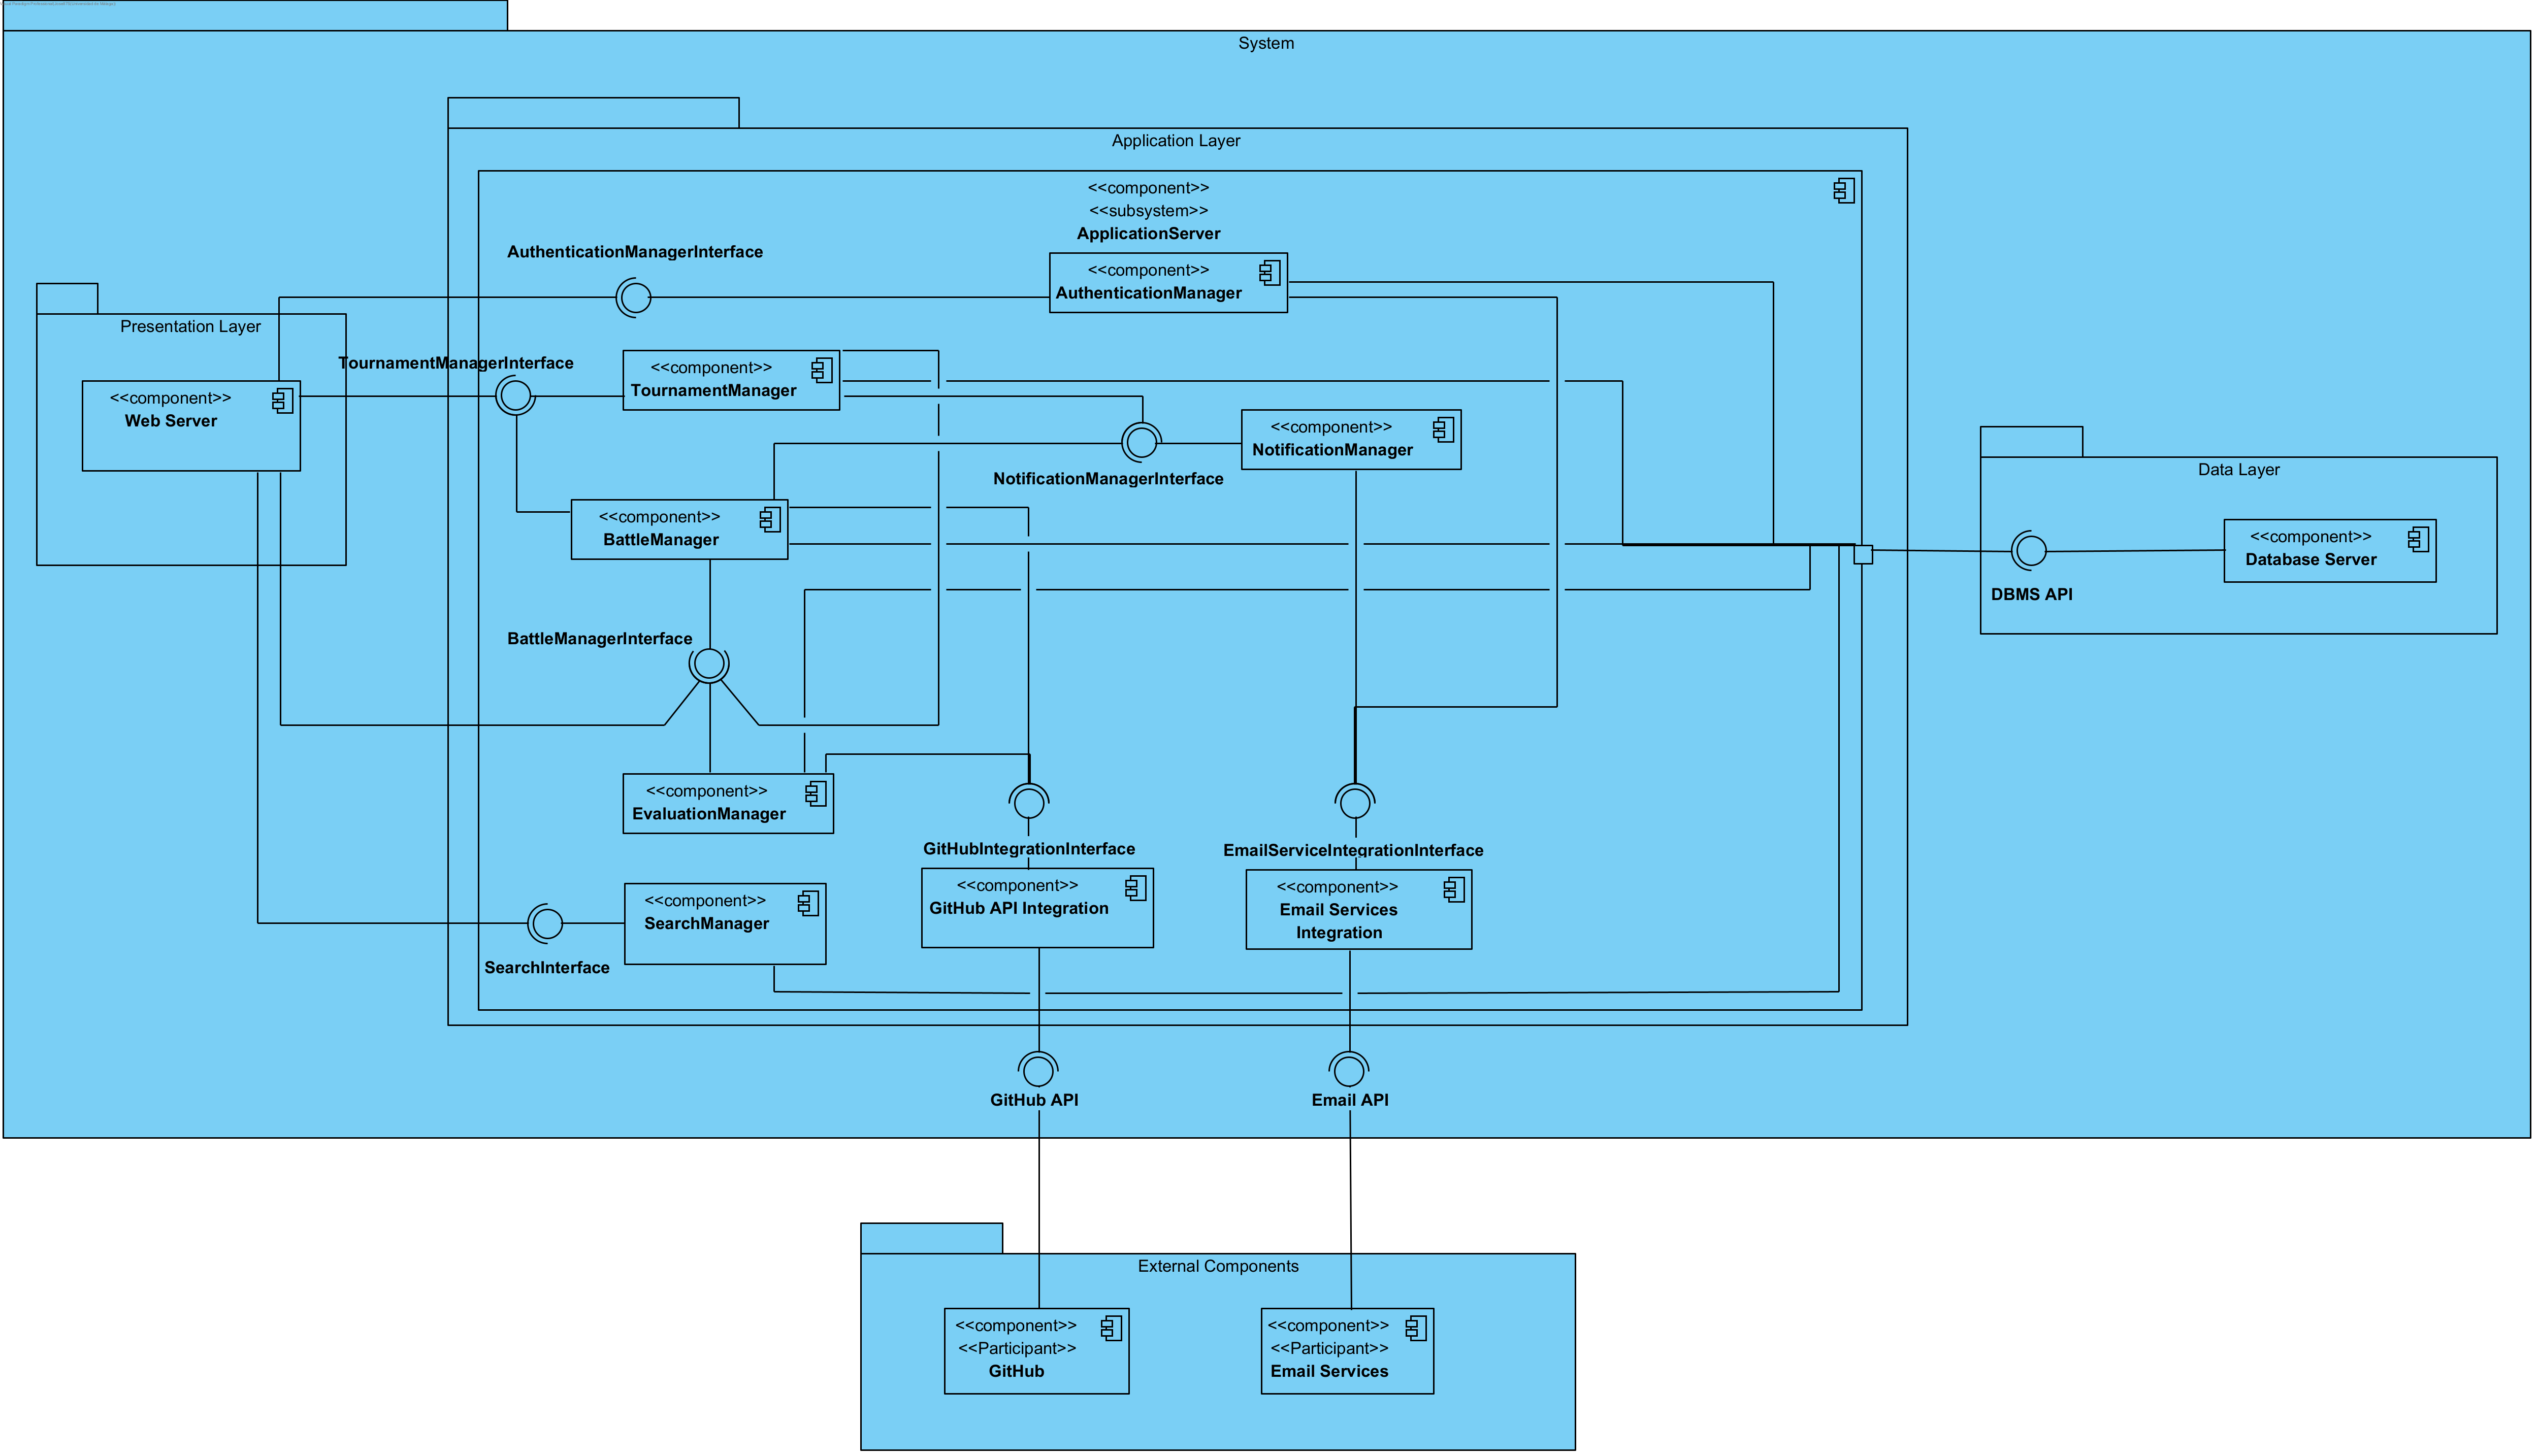
\includegraphics[width=1\textwidth]{images/ComponentDiagram.png}
    \caption{Component Diagram}
    \label{fig:ComponentDiagram}
\end{figure}

\subsubsection{Presentation Layer}

\paragraph{Web Application:}

\begin{itemize}
    \item Represents the web application that will be used by educators and students.
    \item Allows educators to create tournaments and battles, invite other educators to tournaments, and perform manual evaluations on the submissions of battles they own.
    \item Allows students to register to tournaments and battles, create teams, and submit their solutions to battles.
    \item Provides a leaderboard that is updated in real-time, displaying the rankings of participants based on their performance in the battles.
    \item Provides a search functionality that allows users to search for tournaments and battles.
    \item Interfaces with the Web Server for communication with the Application Layer.
\end{itemize}

\paragraph{Web Server:}

\begin{itemize}
    \item Represents the component responsible for hosting the web application.
    \item Handles requests and responses from all users, including educators and students.
    \item Invokes APIs for communication with the Application Layer.
\end{itemize}

\subsubsection{Application Layer}

\paragraph{AuthenticationManager:}

\begin{itemize}
    \item Manages user authentication for educators and students.
    \item Generates and validates authentication tokens.
    \item Interfaces with email services for account confirmation and recovery.
    \item Interfaces with the Data Layer for user authentication.
\end{itemize}

\paragraph{TournamentManager:}

\begin{itemize}
    \item Manages the creation, moderation, and deletion of tournaments.
    \item Handles tournament-related processes and rules.
    \item Interfaces with the BattleManager for battle-related processes such as battle creation.
    \item Interfaces with the Data Layer for tournament data.
\end{itemize}

\paragraph{BattleManager:}

\begin{itemize}
    \item Manages the creation, moderation, and deletion of battles within tournaments.
    \item Handles battle-related processes such as registrations, its deadlines, its GitHub 
    repository creation, and its leaderboard.
    \item Interfaces with the TournamentManager for tournament-related processes such as tournament leadeboard updating.
    \item Interfaces with GitHub API Integration for repository creation.
    \item Interfaces with the Data Layer for battle data.
\end{itemize}

\paragraph{EvaluationManager:}

\begin{itemize}
    \item Handles the evaluation of code submissions based on set criteria.
    \item Utilizes build automation scripts and test cases for evaluation.
    \item Interfaces with the BattleManager for battle-related processes such as battle leadeaboard updating.
    \item Interfaces with GitHub API Integration for repository pulling.
    \item Interfaces with the Data Layer for storage of evaluation results.
\end{itemize}

\paragraph{NotificationManager:}

\begin{itemize}
    \item Manages the sending of notifications to users.
    \item Interfaces with the TournamentManager and BattleManager for tournament and battle-related notifications.
    \item Interfaces with Email Services Integration for sending notifications.
\end{itemize}

\paragraph{SearchManager:}

\begin{itemize}
    \item Manages the search functionality of the platform.
    \item Allows users to search for tournaments and battles.
    \item Interfaces with the Data Layer for tournament and battle data.
\end{itemize}

\subsubsection*{External Components Integration}

\paragraph{GitHub API Integration:}

\begin{itemize}
    \item Interacts with the EvaluationManager to notify of new submissions.
    \item Communicates with the external GitHub API for repository creation and pulling.
\end{itemize}

\paragraph{Email Services Integration:}

\begin{itemize}
    \item Integrates with Email Services for sending notifications.
    \item Sends notifications for tournament invitations, submission updates, etc.
    \item Communicates with the external Email Services API for sending emails.
\end{itemize}

\subsubsection{Data Layer}

\paragraph{Database:}

\begin{itemize}
    \item Manages the storage and retrieval of persistent data.
    \item Stores information related to tournaments, battles, users, submissions, etc.
\end{itemize}


\subsection{Deployment view}

\begin{figure}[H]
    \centering
    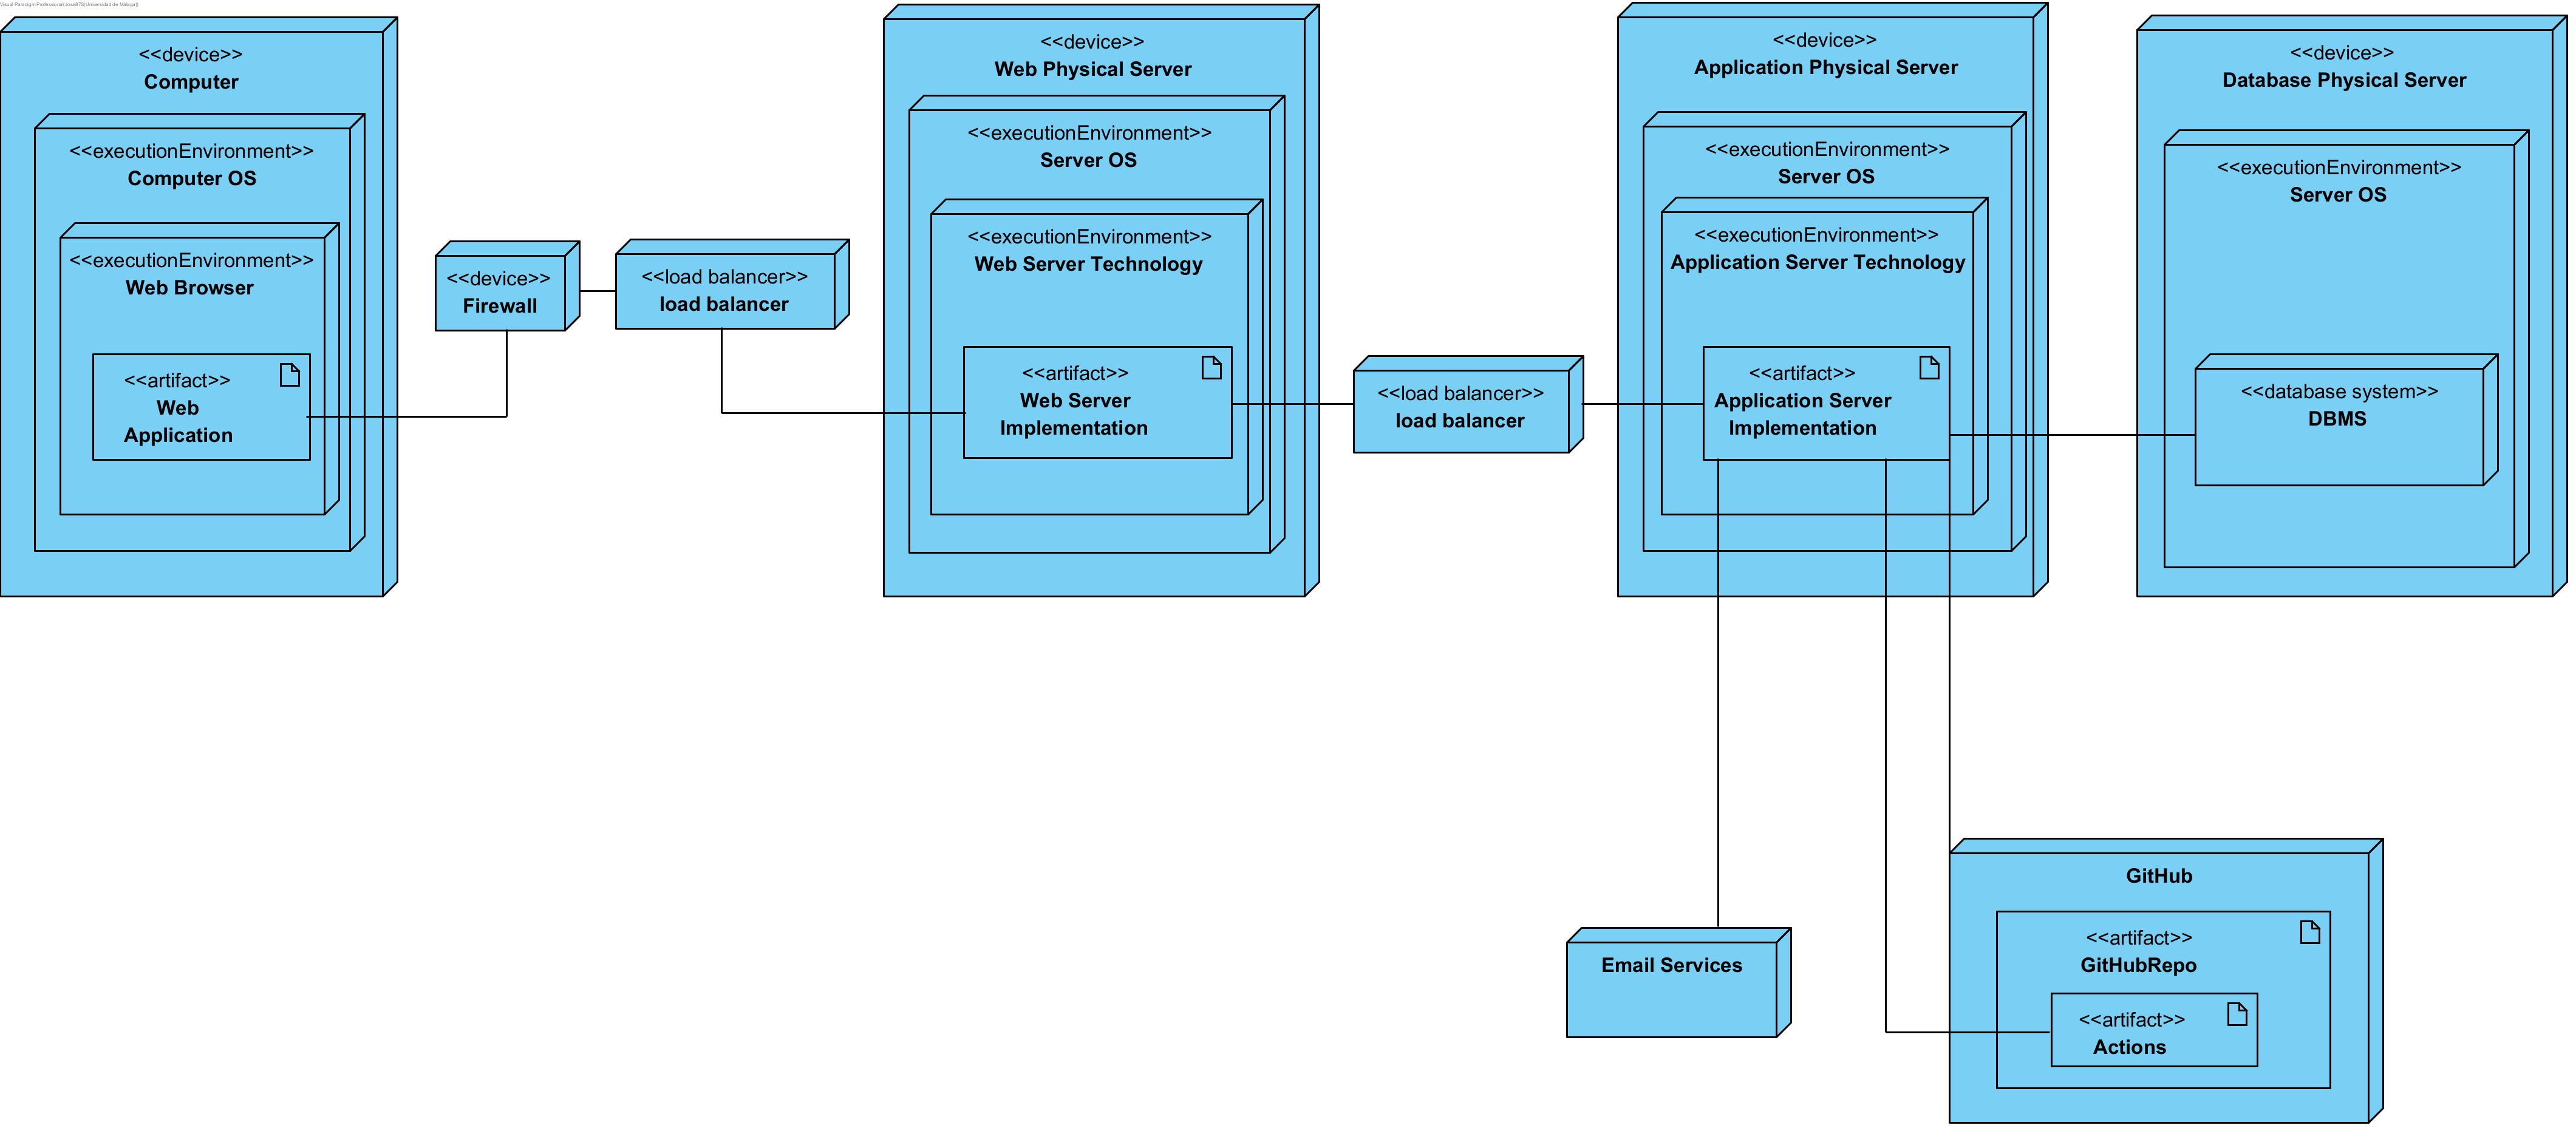
\includegraphics[width=1\textwidth]{images/DeploymentDiagram.png}
    \caption{Deployment Diagram}
    \label{fig:DeploymentDiagram}
\end{figure}

On the deployment diagram, we can see the different components of the system and how they are 
deployed on the different nodes. The web application runs on the users' PC which communicates with the
web server, which runs on a Web Server Technology which could be Apache Tomcat, Nginx or other. This two 
elements represent the presentation layer.
The web server is connected to the application server, which runs on a Java EE Application Server. This
element represents the application layer. The application server is connected to the database and to 
the external components. The database is managed by a Database Management System such as MySQL, PostgreSQL or other. 

\subsection{Runtime view}

In the following diagrams we can see the sequence diagrams of the main functionalities of the system.
These are more fleshed out versions of the use case diagrams presented in the RASD document.

\subsection{Component interfaces}
\subsection{Selected architectural styles and patterns}
\subsection{Other design decisions}

% 3. USER INTERFACE DESIGN
\section{USER INTERFACE DESIGN}

% 4. REQUIREMENTS TRACEABILITY
\section{REQUIREMENTS TRACEABILITY}

% 5. IMPLEMENTATION, INTEGRATION AND TEST PLAN
\section{IMPLEMENTATION, INTEGRATION AND TEST PLAN}

% 6. EFFORT SPENT
\section{EFFORT SPENT}

% 7. REFERENCES
\section{REFERENCES}


\end{document}
